\documentclass[10pt,letterpaper]{article}
\usepackage{amsmath,amssymb,geometry,graphicx}
\usepackage{enumitem}
%\settextfont{B Nazanin}
\usepackage{lipsum}
\setlength{\parskip}{3mm}
\setlength{\parindent}{0mm}
\newcommand{\wid}{0.49\textwidth}
\newcommand{\widone}{60mm}
\begin{document}
\Large
\begin{center}
In the name of beauty

10th problem set of ComNet course

\hrulefill
\end{center}
Q1) Determine the following statements as true or false. (Use enough reasons and explanation to support your answer)

\begin{enumerate}[label=\alph*-]
\item
The hidden terminal problem disappears if no physical obstacle exists in the environment.
\item
For a given modulation scheme, the higher the SNR of a service in physical layer is, the lower its bit error rate will be.
\item
Like Ethernet, ARQ techniques are used in link-layer of a wireless network for coping with high bit error rates.
\item
Addressing a mobile node residing in a foreign network with the approach that the foreign network advertise a highly specific route to the mobile node to the other domains, is a scalable solution that does not require significant changes to the network-layer infrastructure.
\end{enumerate}

Q2) Mention two reasons that why should a \textbf{hand-off} take place in GSM during an ongoing call of a mobile node.

Q3) Figure 1 illustrates a schema for CDMA with two senders.
\begin{figure}[htbp]
\centering
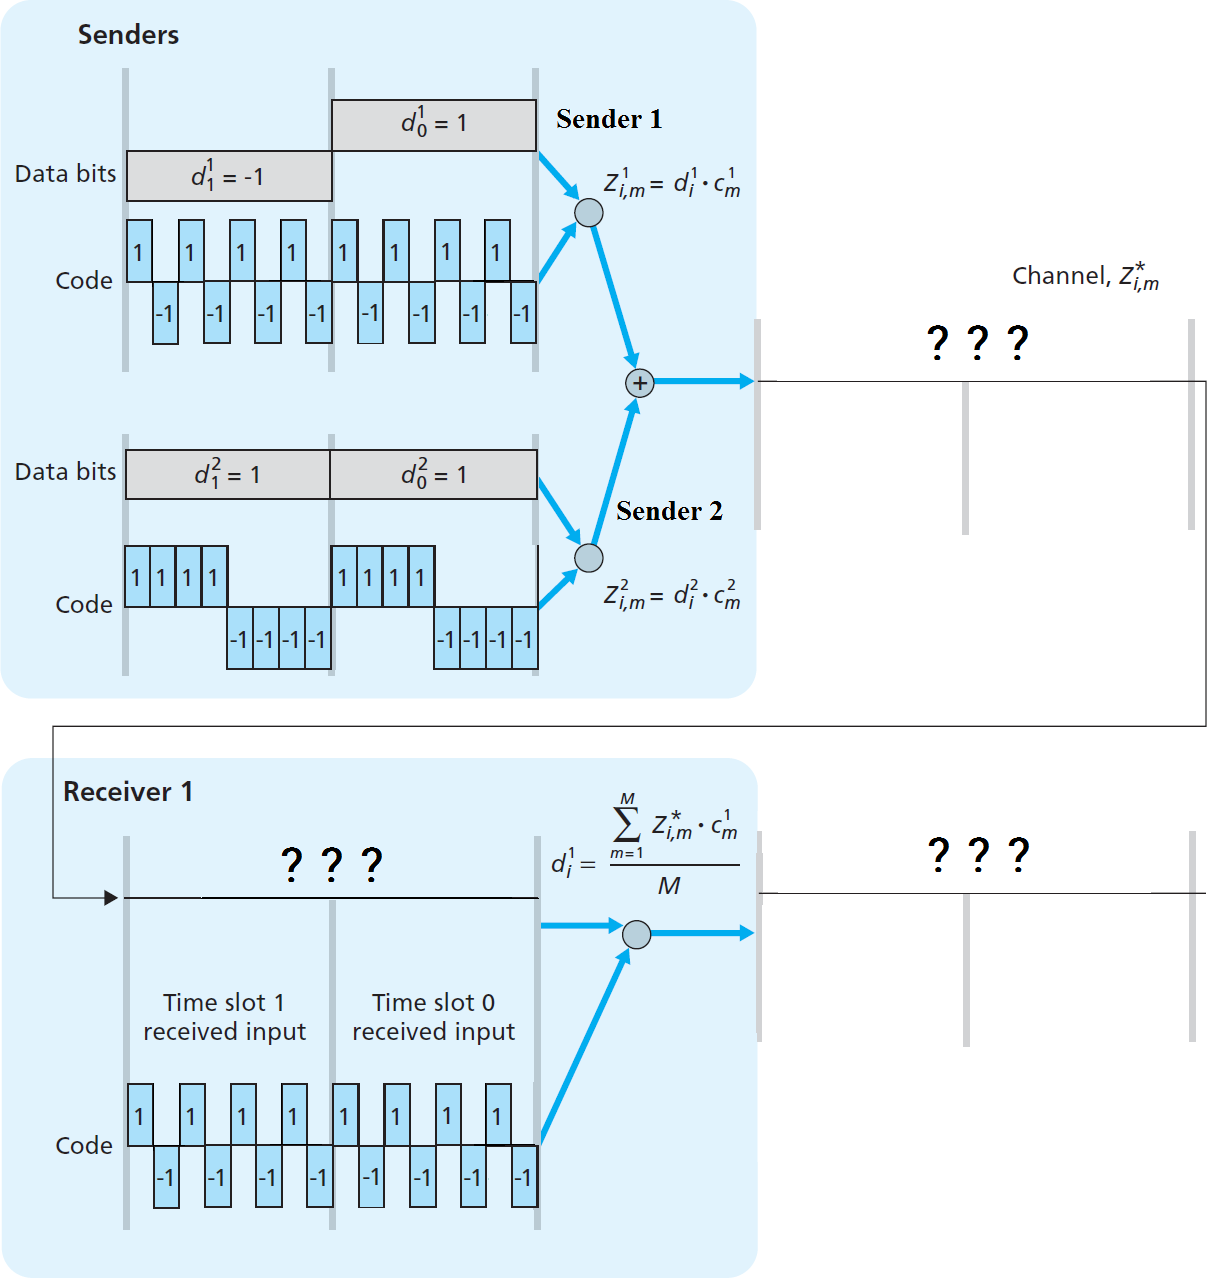
\includegraphics[width=130mm]{CDMA_TXRX.png}
\caption{}
\end{figure}

Each Sender transmits two bits, each of which coded with his own CDMA code (with a chipping rate of 8 times faster than the bit rate).
\begin{enumerate}[label=\alph*-]
\item
Find the strings of $Z_{i,m}^1$, $Z_{i,m}^2$ and $Z_{i,m}^*$.
\item
Assuming that receiver 1 wishes to recover the two bits of sender 1, find $d_1^1$ and $d_0^1$.
\end{enumerate}
(Hints:

The indices $i$ and $m$ in $Z_{i,m}^1$, denote the sender index and the CDMA code bit index, respectively. $c_m^i$ is the CDMA code bit string of the $i$-th sender and the results of $Z_{i,m}^1$, $Z_{i,m}^2$ and $Z_{i,m}^*$ must be 8-bit strings each.

The summations denoted in the figure are NOT modulo-2. They are ordinary summations.

Read the subsection 6.2.1 (CDMA) and the figures 6.5 and 6.6 of the textbook for more explanations, if needed.
)

Q4) \textit{(Extra Points)}

a) Under Ethernet's CSMA/CD, multiple access protocol, a station begins transmitting as soon as the channel is sensed idle. With 802.11 CSMA/CA, however, the station refrains from transmitting while counting down, even when it senses the channel to be idle.Why do CSMA/CD and CDMA/CA take such different approaches here?

b) Consider the 802.11 CSMA/CA once again. Assume that two stations $A$ and $B$ want to send frames. If $A$ and $B$ have experienced $n_A$ and $n_B$ collisions respectively and both, simuletaneously execute the binary exponential back-off for a radom delay before retransmission, what is the probability that the stations $A$ and $B$ do not collide in transmission due to equally generated random delays?

Q5) \textit{(Extra Points)}

Consider Figure 2. Assume that a host $H1$ broadcasts an RTS control frame to all the nodes, including an AP, to further send a DATA frame to another host, say $H2$. The AP, having received the RTS control frame, broadcasts a CTS control frame to $H1$
 which is correctly received by \textbf{all other nodes} in the network, but lost on its way back to $H1$. The host $H1$ waits for a while, then retransmits the RTS control frame. The new RTS control frame is now errorneously detected as DATA in the AP. Explain what happens next.

\begin{figure}[htbp]
\centering
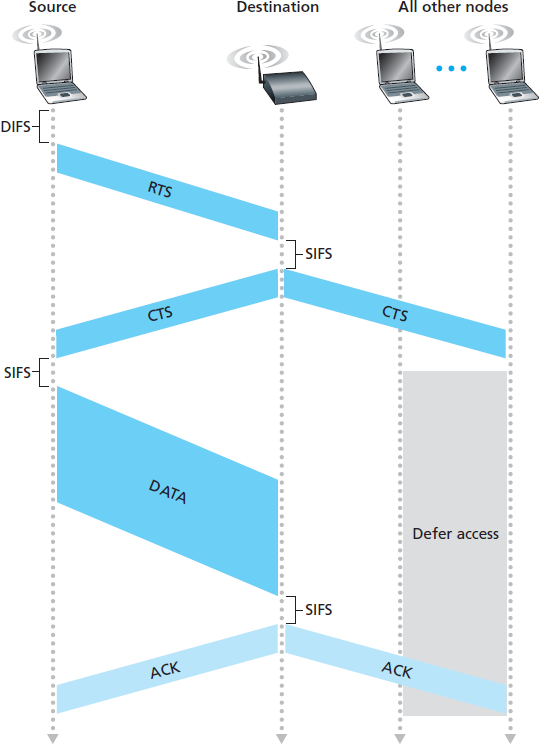
\includegraphics[width=130mm]{CTSRTS.png}
\caption{}
\end{figure}
\end{document}